\documentclass{article}
\usepackage[utf8]{inputenc}
\usepackage{tikz, pgfplots}
\pgfplotsset{compat=1.18,width=10cm}
\usetikzlibrary{positioning}
\title{Graphics}
\begin{document}
\maketitle
\section{Tikz}
\tikz \draw[=>] (0,0) -- (2,1) -- (3,2);
\begin{tikzpicture}
    \draw (0,0) circle (1);
    \draw (2,0) circle(1.5in);
    \draw (5,0) ellipse (10pt and 20pt);
    \draw node at (3,0) {$f(x)$};
\end{tikzpicture}
\vspace{1in}
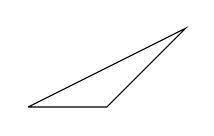
\begin{tikzpicture}
    % \draw (0,0) rectangle (4,2);
    % \draw (0,0) grid(4,2);
    \draw (0,0)--(1,0)--(2,1)--(0,0);
\end{tikzpicture}
\section{2D plots}
\begin{tikzpicture}
    \begin{axis}[xmin=-3,xmax=2,ymin=-3,ymax=3,axis lines=middle,xlabel=$x$,ylabel=$y$,title={Like}]
        \addplot[color=red,dashed,mark=*,samples=10]{x^2};
        \addplot[color=blue]{1-x};
    \end{axis}
\end{tikzpicture}
\\
\begin{tikzpicture}
    \begin{axis}[xmin=0,xmax=2.5*pi,ymin=-1.5,ymax=1.5,axis lines=middle,xlabel=$x$,ylabel=$y$]
        % xtick={0,pi/2,pi,3*pi/2,2*pi},
        % xtickslabel={$0$,$pi/2$,$pi$,$3*pi/2$,$2*pi$},
    \end{axis}
\end{tikzpicture}
\\
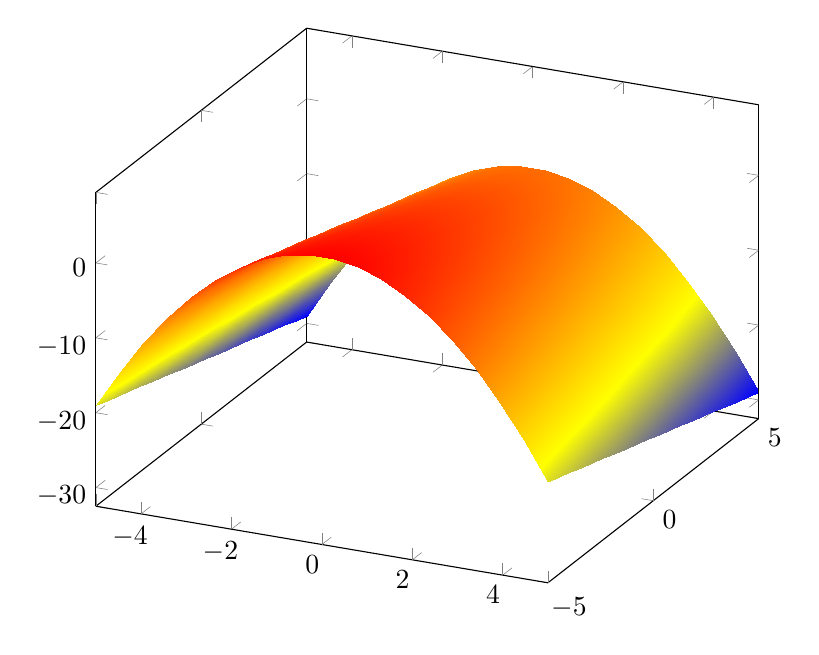
\begin{tikzpicture}
    \begin{axis}
        \addplot3[surf,samples=20,shader=interp]{1-x^2-y};
    \end{axis}
\end{tikzpicture}

\end{document}